\documentclass[12pt]{article}
\usepackage[utf8]{inputenc}
\usepackage{lineno}
\usepackage{authblk}
\usepackage[margin=1in]{geometry}
\usepackage{xparse}
\usepackage{xpunctuate}
\usepackage{xspace}
\usepackage{graphicx}
\usepackage{wrapfig}
\usepackage[hidelinks]{hyperref}
\usepackage[all]{hypcap}
\usepackage{amsmath}
\usepackage{cleveref}
\usepackage{placeins}
\usepackage{flafter}
\usepackage{floatrow}
\usepackage{minted} 
\usepackage{caption}
\usepackage{float}
\usepackage{csvsimple}
\usepackage{booktabs}

% local definitions
\newcommand{\msprime}[0]{\texttt{msprime}\xspace}
\newcommand{\tskit}[0]{\texttt{tskit}\xspace}
\newcommand{\slim}[0]{\texttt{SLiM}\xspace}
\newcommand{\pyslim}[0]{\texttt{pyslim}\xspace}
\newcommand{\allel}[0]{\texttt{scikit-allel}\xspace}
\newcommand*{\eg}{e.g.\xcomma}
\newcommand*{\ie}{i.e.\xcomma}


%\linenumbers

\begin{document}

\title{Bridging forward-in-time and coalescent simulations using pyslim}
\author[1]{Shyamalika Gopalan}
\author[2,3]{Murillo F. Rodrigues}
\author[3,4]{Peter L. Ralph}
%\author[5]{Ben Haller}

\affil[1]{Department of Genetics and Biochemistry and Center for Human Genetics, Clemson University}
\affil[2]{Division of Genetics, Oregon National Primate Center, Oregon Health \& Science University}
\affil[3]{Department of Biology and Institute of Ecology and Evolution, University of Oregon}
\affil[4]{Department of Mathematics, University of Oregon}
%\affil[5]{Department of Computational Biology, Cornell University}

\maketitle

\abstract{
Lorem ipsum
}
\date{}

\section*{Introduction}
% The importance of simulations in popgen and flavors of simulations
Simulations have been an invaluable tool in population genetics for the past six decades.
%because of the difficulty in obtaining analytical solutions to complex evolutionary scenarios.
The two main strategies for population genetic simulation differ in the direction of the process: forward or backward-in-time.
The coalescent process models the ancestry of sampled genomes back in time until they coalesce into one most common recent ancestor (MRCA).
It is perhaps the most common framework for population genetic simulation because of its efficiency:
it bypasses the need to represent entire populations in memory and the sampling of gametes every generation.
Despite its efficiency, the coalescent has strict assumptions (\eg neutrality) which limits applicability.
Forward-in-time simulations starts with actual individuals and applies evolutionary rules (\eg mutation, recombination, selection) over generations until a certain criterion is met.
Thus, forward-in-time simulations are much more flexible, but they come with a high computational cost.

% The tree sequence and its utility in bridging forward-in-time and coalescent simulations
Recent advancements both in computational power and software development have made simulations much more accessible and popular.
A key development that has decreased the computational cost of simulations is the tree sequence,
a data structure that concisely encodes correlated genealogies along the genome.
In the context of forward-in-time simulations,
the recording of tree sequences increases efficiency because it allows for
(i) the omission of neutral mutations during the simulation process, and
(ii) the use of fast coalescent as a neutral "burn-in" phase,
such that the forward simulation can begin with an equilibrium level of genetic diversity.
Further, using tree sequences it is possible to bridge forward and backwards methods, 
for example by using the coalescent to ensure all lineages coalesce into a single common ancestor (a process called \"recapitation\").

% The pyslim package and overview of the chapter
Here, we present \pyslim, a Python package for reading and modifying \tskit tree sequences produced by
the popular coalescent and forward-in-time simulation tools such as \slim and \msprime.
\pyslim provides a way to perform \"hybrid\" simulations, combining both forwards and backwards (coalescent) methods.
We will describe the main uses of \pyslim: (i) recapitation, which is the process of filling in the history of the first-generation individuals which have not coalesced, (ii) generation of initial diversity for forward-in-time simulations, (iii) parallelization of multi-species simulations, and (iv) complex simulation of alternating life cycles.

\section*{Starting with diversity generated by coalescent simulation}

Simulations of large populations with selection can be costly,
especially because we might need to run a lengthy “burn-in” period to get the genetic variation for selection to act on.
Because the precise form of the burn-in may not be important, 
a neutral burn-in can be efficiently run with coalescent simulator such as \msprime.
In this section, we will demonstrate how to perform such a hybrid simulation using \pyslim, \msprime and \slim.

Imagine the scenario where we perform a lab experiment in which
we take high-diversity organisms from the wild and subject them to selection for a few dozen generations.
Although genetic diversity in the wild is most likely not neutral,
we do not know precisely what it does look like and a coalescent simulation would be an acceptable starting point.
The key attribute of reality we would like to approximate is the joint distribution of allele frequencies and effect sizes.
If the alleles affect a trait under stabilizing selection,
we would expect a negative correlation between the two.
On the other hand, there would be no relationship between allele frequencies and effect sizes
if the trait we are selecting on in the lab is not under strong selection in the wild.
We will simulate the scenario where the trait we put under selection in the lab is not under stabilizing selection in the wild.
To do so, we will:

\begin{enumerate}
    \item Run a coalescent simulation with msprime.

    \item Add \slim metadata to the nodes, individuals, and populations.

    \item Add \slim mutations with msprime, and edit the mutation metadata to assign selection coefficients.

    \item Run the \slim portion of the simulation.

    \item Do some descriptive analysis of the results of selection.

    \item Add neutral mutations to the tree sequence.

    \item Do some descriptive analysis of genetic diversity along the genome.
\end{enumerate}

\section*{Parallelizing forward-in-time simulations of multiple species}

Any two branches stemming from the same node in a species tree are independent from each other and
thus can be simulated in parallel (assuming no migration between the species).
For example, in the phylogeny depicted in Figure~\ref{fig:phylo},
branches of the same color can be simulated in parallel.
To do so, we will need to
(i) simulate the history of each branch and
(ii) join the resulting simulations together onto one multi-species history.

 \begin{figure}[h!]
 \centering
  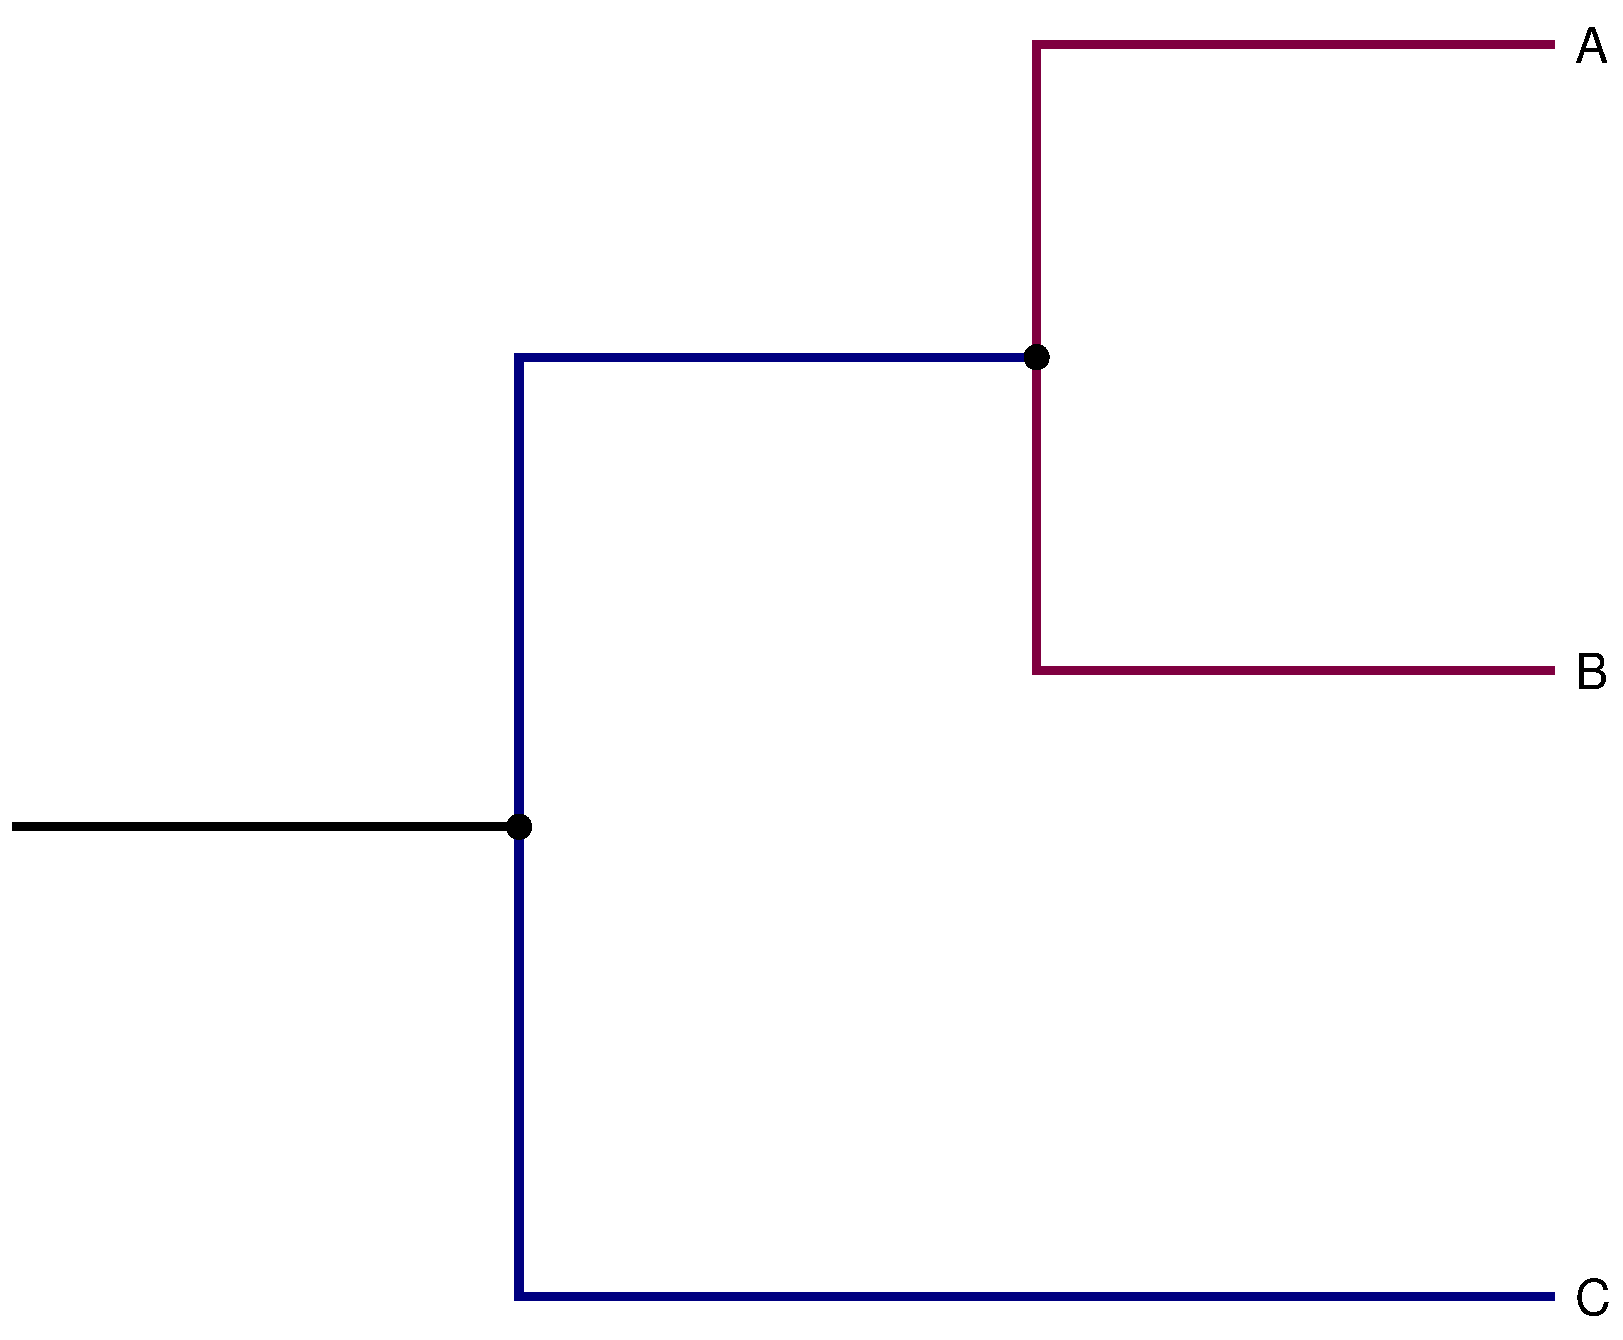
\includegraphics[width=0.5\textwidth]{./code/parallelizing_phylogeny/phylo.pdf}
  \caption{Example of phylogeny we might want to simulate. Note how branches with the same color can be simulated in parallel when there is no migration.}
  \label{fig:phylo}
 \end{figure}

\subsection{Parallel simulation of branches}

First, we need to write a \slim script that will be used for simulating the history of each branch in our phylogeny.
We will perform a simple simulation,
in which each branch can have a different (but fixed) population size and length (number of ticks).
Also, we will allow deleterious mutations to happen across the entire chromosome at a fixed rate.
See the code below (Listing~\ref{lst:slim-example}).

\begin{listing}[H]
  \inputminted[fontsize=\small, linenos, bgcolor=gray!10]{javascript}{./code/parallelizing_phylogeny/simulate_branch.slim}
  \caption{Simple \slim script to simulate a constant size population that can be started from an existing tree sequence.}
  \label{lst:slim-example}
\end{listing}

For each branch, the presence or absence of \verb|infile| tells \slim whether a previous branch exists or not.
If so, \slim will read the previous tree sequence and change the population size accordingly.
Note that when you read a tree sequence into \slim,
the tick counter will be updated with the time encoded in the tree sequence,
so we need to set the end of the simulation as the length of the branch (\verb|num_gens|)
plus the current “time” at the end of the loaded tree sequence.
At the end of the simulation, we call \verb|sim.treeSeqRememberIndividuals| right before saving the resulting tree sequence.
This is necessary because we need to ensure the individuals in the final generation are never dropped
from the tree sequence in future runs of \slim which are started from the output of the simulation,
as they will later be used to glue the tree sequences together.

The example phylogeny we will simulate is encoded in the table below (Table~\ref{tab:phylo}).

\begin{table}[H]
  \centering
  \caption{Parameters of the phylogeny that will be simulated.}
  \label{tab:phylo}
    \begin{tabular}{llll}
      \bfseries Child & \bfseries Parent & \bfseries Population size & \bfseries Edge length \\
      \hline
      \csvreader[head to column names]{./code/parallelizing_phylogeny/phylo.csv}{}%
        {\child & \parent & \popsize & \edgelen\\}
    \end{tabular}
\end{table}

\end{document}
